\documentclass[tikz,border=2pt]{standalone}
\usetikzlibrary{arrows.meta,automata,positioning}
\usepackage{siunitx} 

\begin{document}
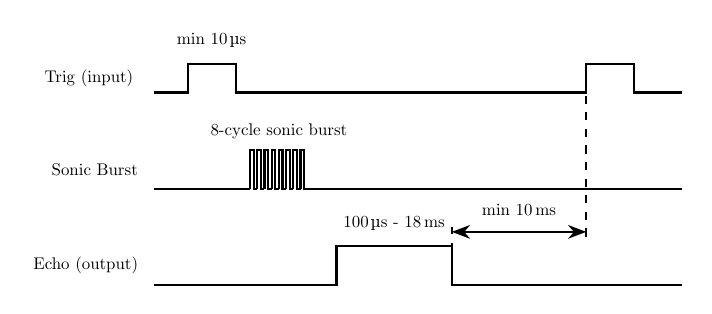
\begin{tikzpicture}[scale=0.61, transform shape,thick,>=Stealth]

% =====================
% Livelli verticali
% =====================
\def\TrigY{4}
\def\SonicY{2}
\def\EchoY{0}

% =====================
% Trigger input
% =====================
\draw
(0,\TrigY) -- (0.7,\TrigY)
-- (0.7,\TrigY+0.6) -- (1.7,\TrigY+0.6)
-- (1.7,\TrigY) -- (7+2,\TrigY)
-- (7+2,\TrigY+0.6) -- (8+2,\TrigY+0.6)
-- (8+2,\TrigY) -- (9+2,\TrigY);

\node[left] at (-0.3,\TrigY+0.3) {Trig (input)};
\node[above=0.2cm] at (1.2,\TrigY+0.6) {min $10\,\si{\micro\s}$};

% =====================
% Sonic burst
% =====================
\draw (0,\SonicY) -- (2,\SonicY);

\foreach \x in {2,2.15,...,3.1} {
  \draw (\x,\SonicY) -- (\x,\SonicY+0.8) --
  (\x+0.075,\SonicY+0.8) -- (\x+0.075,\SonicY) -- (\x+0.15,\SonicY);
}

\draw (3.1,\SonicY) -- (9+2,\SonicY);

\node[left, text width=2cm] at (0,\SonicY+0.4) {Sonic Burst};
\node[above] at (2.6,\SonicY+0.9) {8-cycle sonic burst};

% =====================
% Echo pulse
% =====================
\draw (0,\EchoY) -- (3.8,\EchoY)
-- (3.8,\EchoY+0.8) -- (6.2,\EchoY+0.8)
-- (6.2,\EchoY) -- (9+2,\EchoY);

\node[left] at (-0.2,\EchoY+0.4) {Echo (output)};
\node[above=0.2cm] at (5,\EchoY+0.8) {$100\,\si{\micro\s}$ - $18\,\si{m\s}$};

% =====================
% Timing note
% =====================
\draw[<->]
(6.2,1.1) -- (9,1.1)
node[midway,above=0.2cm]{min $10\,\si{m\s}$};

\draw[dashed] (6.2,\EchoY+0.7) -- (6.2,\EchoY+1.2);
\draw[dashed] (9,\EchoY+1) -- (9,\TrigY);

\end{tikzpicture}
\end{document}
